\section{Evaluation}

In this section, we take table~\ref{tab:background-comparison} from
page~\pageref{tab:background-comparison} as a starting point and check what
features are implemented and what are not.

The testing environment was built from a client machine, a SharePoint server
and an Alfresco server:

\begin{figure}[H]
\centering
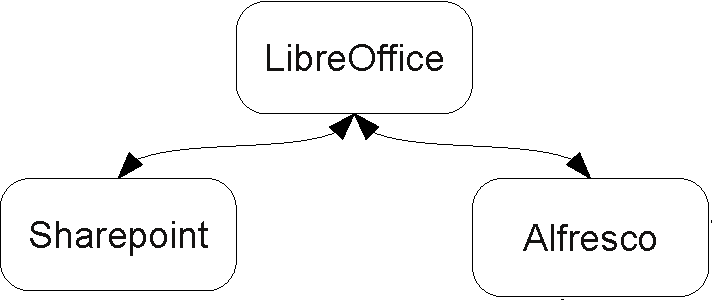
\includegraphics[width=300px,keepaspectratio]{test-arch.pdf}
\caption{Architecture of the test system}
\end{figure}

The client machine had the following details:
\begin{itemize}
\item Hostname: s12
\item Frugalware Linux 1.4 (English and Hungarian locale)
\item LibreOffice 3.3, OpenOffice.org 3.3 and OpenOffice.org 3.2.1
\end{itemize}

Properties of the SharePoint machine:

\begin{itemize}
\item Hostname: vmiklos-sp
\item Microsoft Windows Windows Server 2003 R2 Enterprise (English)
\item Microsoft SharePoint 2007 Enterprise
\end{itemize}

Finally the Alfresco machine:

\begin{itemize}
\item Hostname: diploma1-f
\item Fedora Linux 15 Beta
\item Alfresco 3.4.d Community Edition
\end{itemize}

Regarding functionality, all items from the feature table are implemented in
the extension. The following areas are missing from the table, and not
supported at the moment:

\begin{itemize}
\item User management, including roles and permissions inside workspaces.
\item Task management in workspaces.
\item Link management in workspaces.
\item Creating and deleting workspaces is supported, but nested folder
structures can only be read by the extension.
\end{itemize}

The extension is written in Java and BASIC, so it is meant to be portable.
LibreOffice is available on Windows and OSX as well -- so the extension should
work there, but this is not something we had time to test.

Regarding localization, all user-visible strings are externalized to Java
property files. During development we paid attention to English strings, then at
the end as a demonstration we created the Hungarian translation as well. Adding
new translations is easy.

Finally, the extension inherited some of its limitation from the original OPAL
codebase:

\begin{itemize}
\item We decided not to bother with renaming namespaces, so untouched code still
lives under \emph{fr.starxpert}, which may cause a problem if one wants to use
my extension and OPAL at the same time.
\item The \emph{commons-httpclient} jar is still part of the project, though it is not used in fact.
\item The GUI is not started in a separate thread in all cases, resulting the
lack of the update of the user interface background in many cases.
\item Classes we did not touch still have French comments inside.
\end{itemize}
